\chapter{Exemplos e resultados}
\label{chap:exemploseresultados}

Neste capítulo são apresentados os resultados de aplicação da técnica proposta nesse trabalho em alguns modelos. É mostrada a diferença da sua utilização na remoção de ruídos de um modelo. Os resultados para a técnica descrita neste trabalho são nomeados como \textit{pre-guided} e comparados com os resultados obtidos pelos trabalhos de \cite{zhang2015guided}, \cite{sun2007fast} e \cite{zheng2011bilateral}, que serão denotados como \textit{guided}, \textit{fast-and-effective} e \textit{bilateral-normal-filtering}.

A técnica descrita neste trabalho foi implementada em C++, utilizando a biblioteca de API gráfica livre \textit{modern OpenGL} (Open Graphics Library), libigl (https://github.com/libigl/libigl), GLEW, glfw e assimp.

O computador utilizado para a técnica foi um MacBook Air, com processador Intel Core i5, 1.3 GHz, 8 GB de memória DDR3 1600 MHz e placa de vídeo Intel HD Graphics 5000 com 1546 MB de memória gráfica.

\section{Modelos}

Ao todo, foram utilizados 4 modelos, sendo 3 modelos com ruído artificial e regiões com triangulação de baixa qualidade e 1 modelo digitalizado do mundo real para mostrar a eficiência da técnica em problemas reais. Eles serão referidos como: \textit{block}, \textit{carter}, \textit{mechanic} e \textit{angel} (Figura \ref{fig:models}). 

\begin{figure}[!h]
\captionsetup{width=\linewidth}
\centering
\includegraphics[width=\linewidth]{figuras/models.png}
\caption{Modelos utilizados na técnica proposta. Na primeira metade da imagem temos \textit{block} e \textit{carter}, seguidos do modelo \textit{mechanic} em duas visões diferentes. Mais a direita temos o modelo \textit{angel} que foi digitalizado do mundo real a partir de um \textit{scanner} 3D.}
\label{fig:models}
\end{figure}

\begin{figure}[!h]
\captionsetup{width=\linewidth}
\centering 
\includegraphics[scale=0.34]{figuras/artificialnoise.png}
\caption{Processo de criação dos modelos de entrada. A esquerda temos os modelos \textit{ground-truth}: \textit{block}, \textit{carter} e \textit{mechanic} em duas visões diferentes. As regiões em destaque representam a zona onde a qualidade de triangulação foi propositalmente reduzida. A direita tem-se o segundo passo da criação dos modelos artificiais: a aplicação de um ruído branco aleatório e artificial ao longo das normais dos vértices.}
\label{fig:artificialnoise}
\end{figure}

Para mostrar a robustez da técnica apresentada, utilizamos dois processos na criação dos 3 primeiros modelos de entrada:
\begin{itemize}
    \item Algumas regiões do modelo foram reconstruídas, deixando a triangulação com qualidade ruim.
    \item Um processo de ruído artificial é aplicado. Os vértices são movidos a uma pequena distância aleatória (positiva ou negativa) na direção da sua normal.
\end{itemize}

Ao final deste processo, ilustrado na Figura \ref{fig:artificialnoise}, terão-se os 3 modelos com as duas pré-condições suficientes para que a técnica proposta mostre bons resultados em relação às demais. 

\section{Métricas de Qualidade}\label{metrics}

Para medir qualidade e eficiência em uma técnica de remoção de ruídos, a grande maioria dos artigos na literatura seguem o seguinte padrão:
\begin{itemize}
    \item Uma malha sem ruído, chamada \textit{ground-truth}, é adquirida.
    \item É aplicado um ruído sintético na \textit{ground-truth}.
    \item A técnica é aplicada obtendo uma malha resultante.
    \item Métricas de comparação são executadas entre a malha resultante e a \textit{ground-truth}.
\end{itemize}

Dessa forma, é medido o quão semelhante a malha resultante ficou da sua forma esperada. Uma forma de medir essa semelhança é calcular a proximidade da malha resultante com a \textit{ground-truth}.

A métrica de qualidade mais comum na literatura é a \textit{distância de erro média} (MDE), definida para uma malha resultante $X$ e uma malha \textit{ground-truth} $G$, pela seguinte equação:
\begin{equation}
    MDE(X,G) = \frac{1}{n} \sum_{i=1}^{n}{\|x_i - g_i \|}, 
\end{equation}
onde $n$ é o número de vértices em ambas as malhas, $x_i$ é um vértice da malha resultante e $g_i$ é o mesmo vértice na malha \textit{ground-truth}. Essa métrica simplesmente calcula a distância média que cada vértice está do resultado ideal (\textit{ground-truth}). Quanto mais próximo o $MDE(X,G)$ estiver de $0$, mais eficiente será a técnica. Como a técnica proposta tem um passo de pré-processamento, em geral a malha resultante vai possuir mais vértices do que a malha \textit{ground-truth}, então essa métrica não deve ser usada diretamente, pois estariam-se ignorando informações relevantes na medida de erro.

Para este fim, como medida de qualidade, foi usado a técnica presente em \cite{cignoni1998metro} para estimar o erro em nosso processo de remoção de ruídos. Esta técnica faz amostragens de pontos na superfície da malha resultante e calcula a distância mínima entre esses pontos e a malha \textit{ground-truth} basedo na distância de \textit{Hausdorff}.

A distância de \textit{Hausdorff}, ilustrada na Figura \ref{fig:hausdorffdistance}, mede o quão distante dois conjuntos de um espaço métrico estão um do outro. Seja $X$ e $Y$ dois subconjuntos não vazios de um espaço métrico. A distância de \textit{Hausdorff} $d_H(X,Y)$ é definida por:
\begin{equation}
	d_H(X,Y) = \max \{ {\sup_{x \in X}} \: {\inf_{y \in Y}} \: d(x,y), \underset{y \in Y}{\sup} \: \underset{x \in X}{\inf} \: d(x,y) \},
\end{equation}
onde $sup$ representa o \textit{supremum}, $inf$ o \textit{infimum} e $d(x,y)$ representa a distância entre os pontos $x \in X$ e $y \in Y$.

\begin{figure}[!h]
\captionsetup{width=\linewidth}
\centering
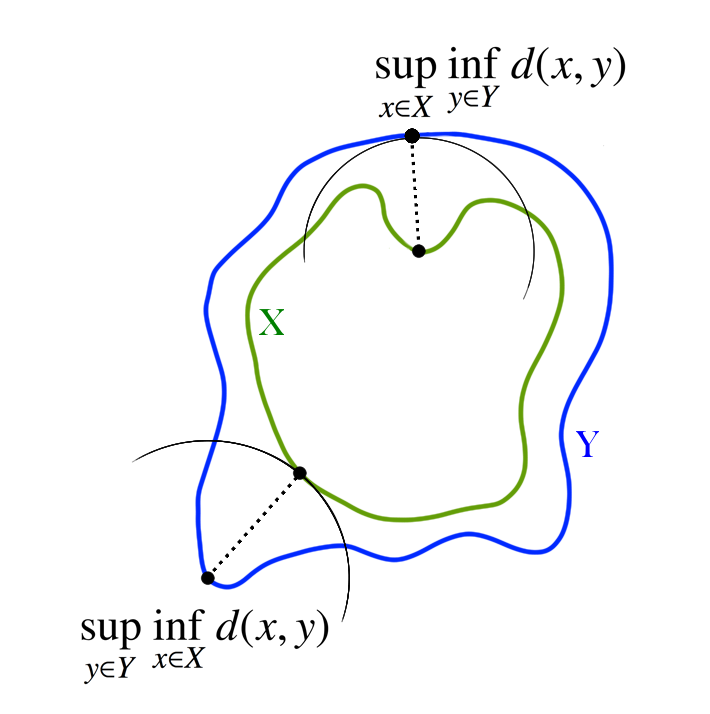
\includegraphics[scale=0.4]{figuras/Hausdorff_final.png}
\caption{A distância de \textit{Hausdorff} entre dois subconjuntos $X$ e $Y$: $d_H(X,Y)$ irá resultar na maior das duas distâncias.}
\label{fig:hausdorffdistance}
\end{figure}

A distância de \textit{Hausdorff} $d_H(X,Y)$ é um valor que representa a distância entre dois subconjuntos. Já que estamos interessados na distância mínima entre cada ponto amostrado na malha resultante, a distância de \textit{Hausdorff} modificada (MHD) para um ponto amostrado $x$ na malha resultante $X$ e a malha \textit{ground-truth} $G$, será definido por:
\begin{equation}
	MHD(x,G) = \underset{g \in G}{\inf} \: d(x,g),
\end{equation}
onde $g$ é o ponto na superfície da malha $G$ que produz a menor distância para $x$. Portanto $MHD(x,G)$ será o resultado da menor distância de um ponto $x$ para a malha $G$. 

Estendendo este conceito para todos os pontos amostrados: seja $n_s$ o número de pontos amostrados na superfície da malha $X$, $x_i$ um ponto amostrado na superfície de $X$ e $g$ o ponto na superfície da malha $G$ que produz a menor distância para $x_i$. Será definida então a distância de \textit{Hausdorff} modificada média (MMHD):
\begin{equation} \label{eq:mmhd}
	MMHD(X,G) = \frac{1}{n_s} \sum_{i=1}^{n_s}{MHD(x_i,G)},
\end{equation}
que conterá a média entre todos os MHD dos pontos amostrados, representando assim a média da distância que a malha resultante está da malha ideal (\textit{ground-truth}).

Apesar da $MMHD$ ser uma métrica mais precisa, irá se usar também a razão entre os volumes da malha resultante e da \textit{ground-truth} para informações mais concisas e completas sobre a validez da técnica proposta. Ao todo serão usadas quatro métricas:

\begin{itemize} 
    \item \textbf{MHD mínimo}: O menor valor de MHD entre todos os pontos amostrados. Esse valor representa o deslocamento mínimo de um ponto na malha resultante causado pela técnica. Valores próximos ou iguais a 0 são preferíveis.
    \item \textbf{MHD máximo}: O maior valor de MHD entre todos os pontos amostrados. Esse valor representa o deslocamento máximo de um ponto na malha resultante causado pela técnica. Valores próximos ou iguais a 0 são preferíveis.
    \item \textbf{MMHD}: O valor médio de todos os valores de MHD dos pontos amostrados como definido em \ref{eq:mmhd}. Valores próximos ou iguais a 0 são preferíveis. Esta é a métrica mais importante.
    \item \textbf{Proporção de Volume}: A razão de proporção entre o volume do modelo resultante e o volume do modelo \textit{ground-truth}. Quanto mais próximo esse valor for de 1, melhor.
\end{itemize}


\section{Resultados}
\label{sec:resultados}

Na sequência, será comparado a técnica proposta com \cite{zhang2015guided}, \cite{sun2007fast} e \cite{zheng2011bilateral}, aplicando as quatro técnicas nos modelos de ruído sintético mostrados na Figura \ref{fig:models}, e utilizando as quatro medidas de qualidade descritas na seção \ref{metrics} para comparação. Todos os modelos foram amostrados com 6000000 de pontos na sua superfície para o cálculo do MMHD. As Figuras \ref{fig:block_final}, \ref{fig:carter_final}, \ref{fig:mechanic1_final} e \ref{fig:mechanic2_final} mostram os resultados finais das técnicas citadas aplicadas aos quatro modelos propostos, mostrando assim a comparação da técnica proposta nesse trabalho com as demais. As Figuras \ref{fig:block_hausdorff_final}, \ref{fig:carter_hausdorff_final}, \ref{fig:mechanic1_hausdorff_final} e \ref{fig:mechanic2_hausdorff_final} ilustram a visualização das distâncias de \textit{Hausdorff} dos 6 milhões de pontos amostrados, assim como um histograma de distribuição desses pontos. O modelo \textit{angel}, que possui ruído real, não possui uma malha \textit{ground-truth} de comparação, portanto usou-se a técnica proposta para mostrar que visualmente ele possui uma melhor qualidade, como é notado nas Figuras \ref{fig:angel_final} e \ref{fig:angel_detail}.



\begin{figure}[p]
\captionsetup{width=\linewidth}
\centering
\includegraphics[width=16cm]{figuras/block_final.png}
\caption{Comparação da técnica proposta com as técnicas de \cite{zhang2015guided}, \cite{sun2007fast} e \cite{zheng2011bilateral} para o modelo \textit{block}. Primeira linha: \textit{ground-truth}, \textit{ground-truth} com malha, modelo com ruído sintético, modelo com ruído sintético e malha. Segunda linha: técnicas de \cite{zhang2015guided}, \cite{sun2007fast}, \cite{zheng2011bilateral} e a técnica proposta, respectivamente. Terceira linha: as mesmas técnicas da linha anterior mostrando as malhas dos modelos.}
\label{fig:block_final}
\end{figure}

\clearpage

\begin{figure}[p]
\captionsetup{width=\linewidth}
\centering
\includegraphics[width=16cm]{figuras/carter_final.png}
\caption{Comparação da técnica proposta com as técnicas de \cite{zhang2015guided}, \cite{sun2007fast} e \cite{zheng2011bilateral} para o modelo \textit{carter}. Primeira linha: \textit{ground-truth}, \textit{ground-truth} com malha, modelo com ruído sintético, modelo com ruído sintético e malha. Segunda linha: técnicas de \cite{zhang2015guided}, \cite{sun2007fast}, \cite{zheng2011bilateral} e a técnica proposta, respectivamente. Terceira linha: as mesmas técnicas da linha anterior mostrando as malhas dos modelos.}
\label{fig:carter_final}
\end{figure}

\clearpage

\begin{figure}[p]
\captionsetup{width=\linewidth}
\centering
\includegraphics[width=16cm]{figuras/mechanic1_final.png}
\caption{Comparação da técnica proposta com as técnicas de \cite{zhang2015guided}, \cite{sun2007fast} e \cite{zheng2011bilateral} para o modelo \textit{mechanic}. Primeira linha: \textit{ground-truth}, \textit{ground-truth} com malha, modelo com ruído sintético, modelo com ruído sintético e malha. Segunda linha: técnicas de \cite{zhang2015guided}, \cite{sun2007fast}, \cite{zheng2011bilateral} e a técnica proposta, respectivamente. Terceira linha: as mesmas técnicas da linha anterior mostrando as malhas dos modelos.}
\label{fig:mechanic1_final}
\end{figure}

\begin{figure}[p]
\captionsetup{width=\linewidth}
\centering
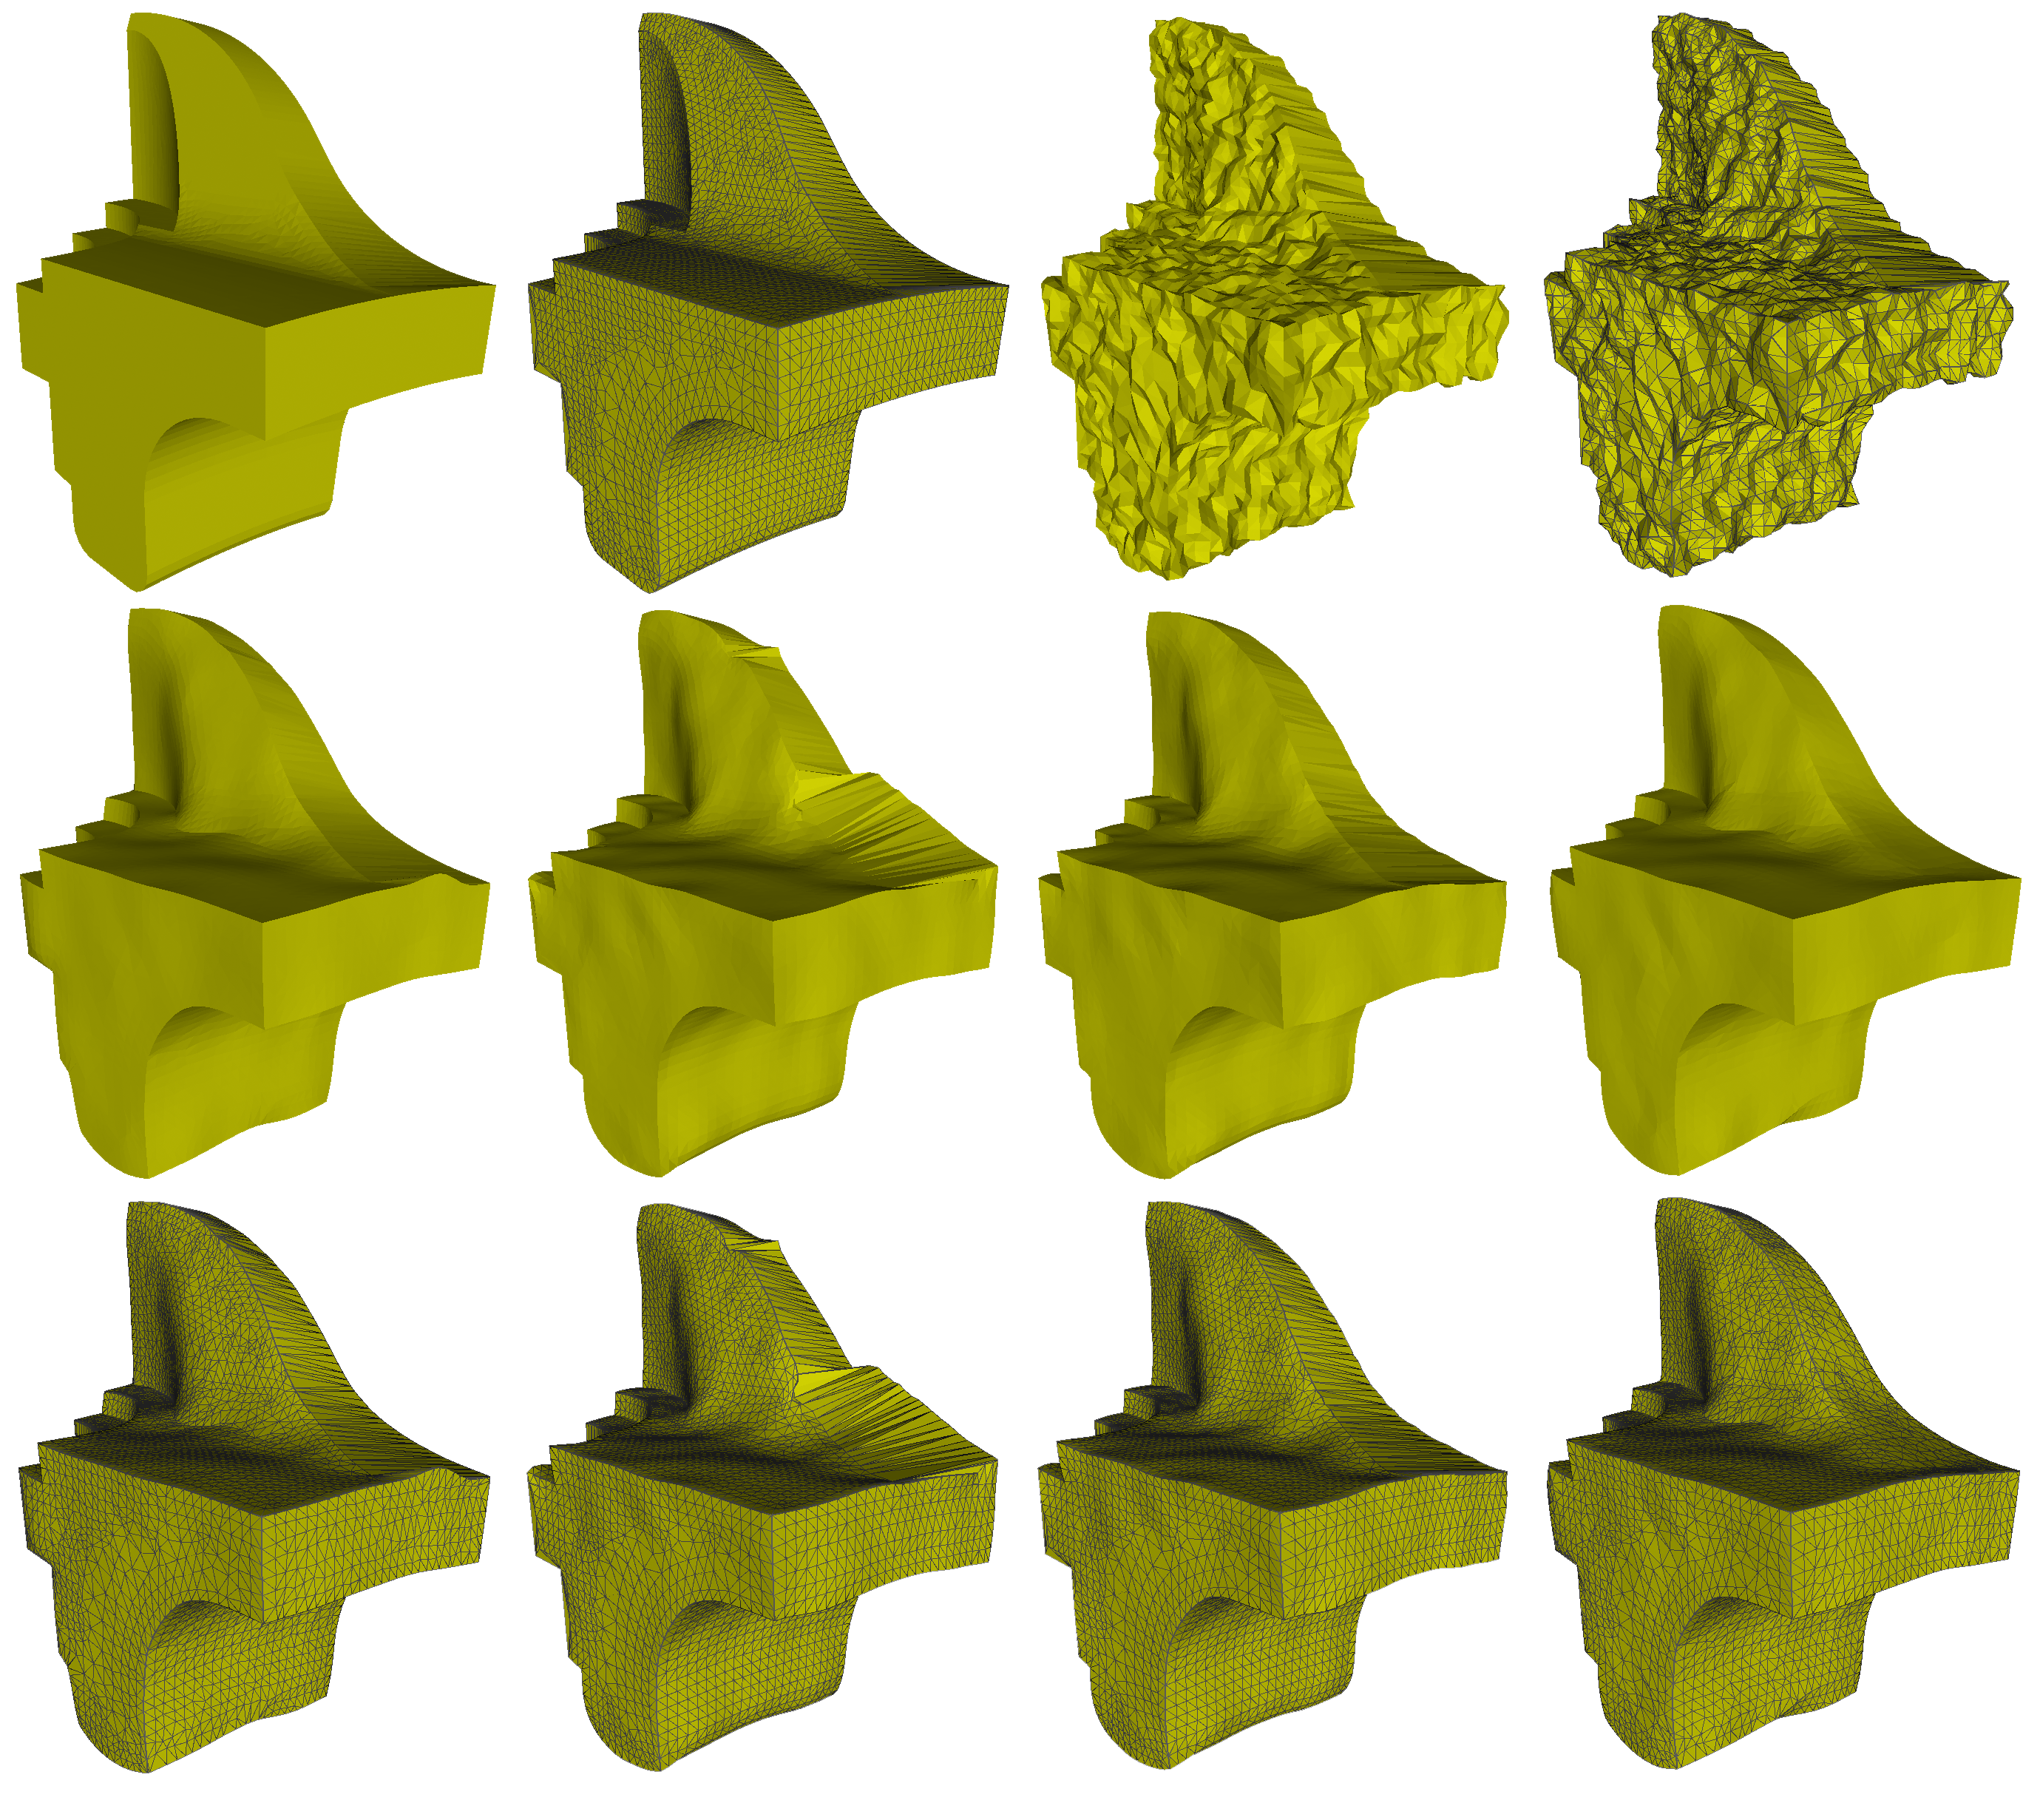
\includegraphics[width=16cm]{figuras/mechanic2_final.png}
\caption{Comparação da técnica proposta com as técnicas de \cite{zhang2015guided}, \cite{sun2007fast} e \cite{zheng2011bilateral} para o modelo \textit{mechanic}. Primeira linha: \textit{ground-truth}, \textit{ground-truth} com malha, modelo com ruído sintético, modelo com ruído sintético e malha. Segunda linha: técnicas de \cite{zhang2015guided}, \cite{sun2007fast}, \cite{zheng2011bilateral} e a técnica proposta, respectivamente. Terceira linha: as mesmas técnicas da linha anterior mostrando as malhas dos modelos.}
\label{fig:mechanic2_final}
\end{figure}

\clearpage






\begin{figure}[p]
\captionsetup{width=\linewidth}
\centering
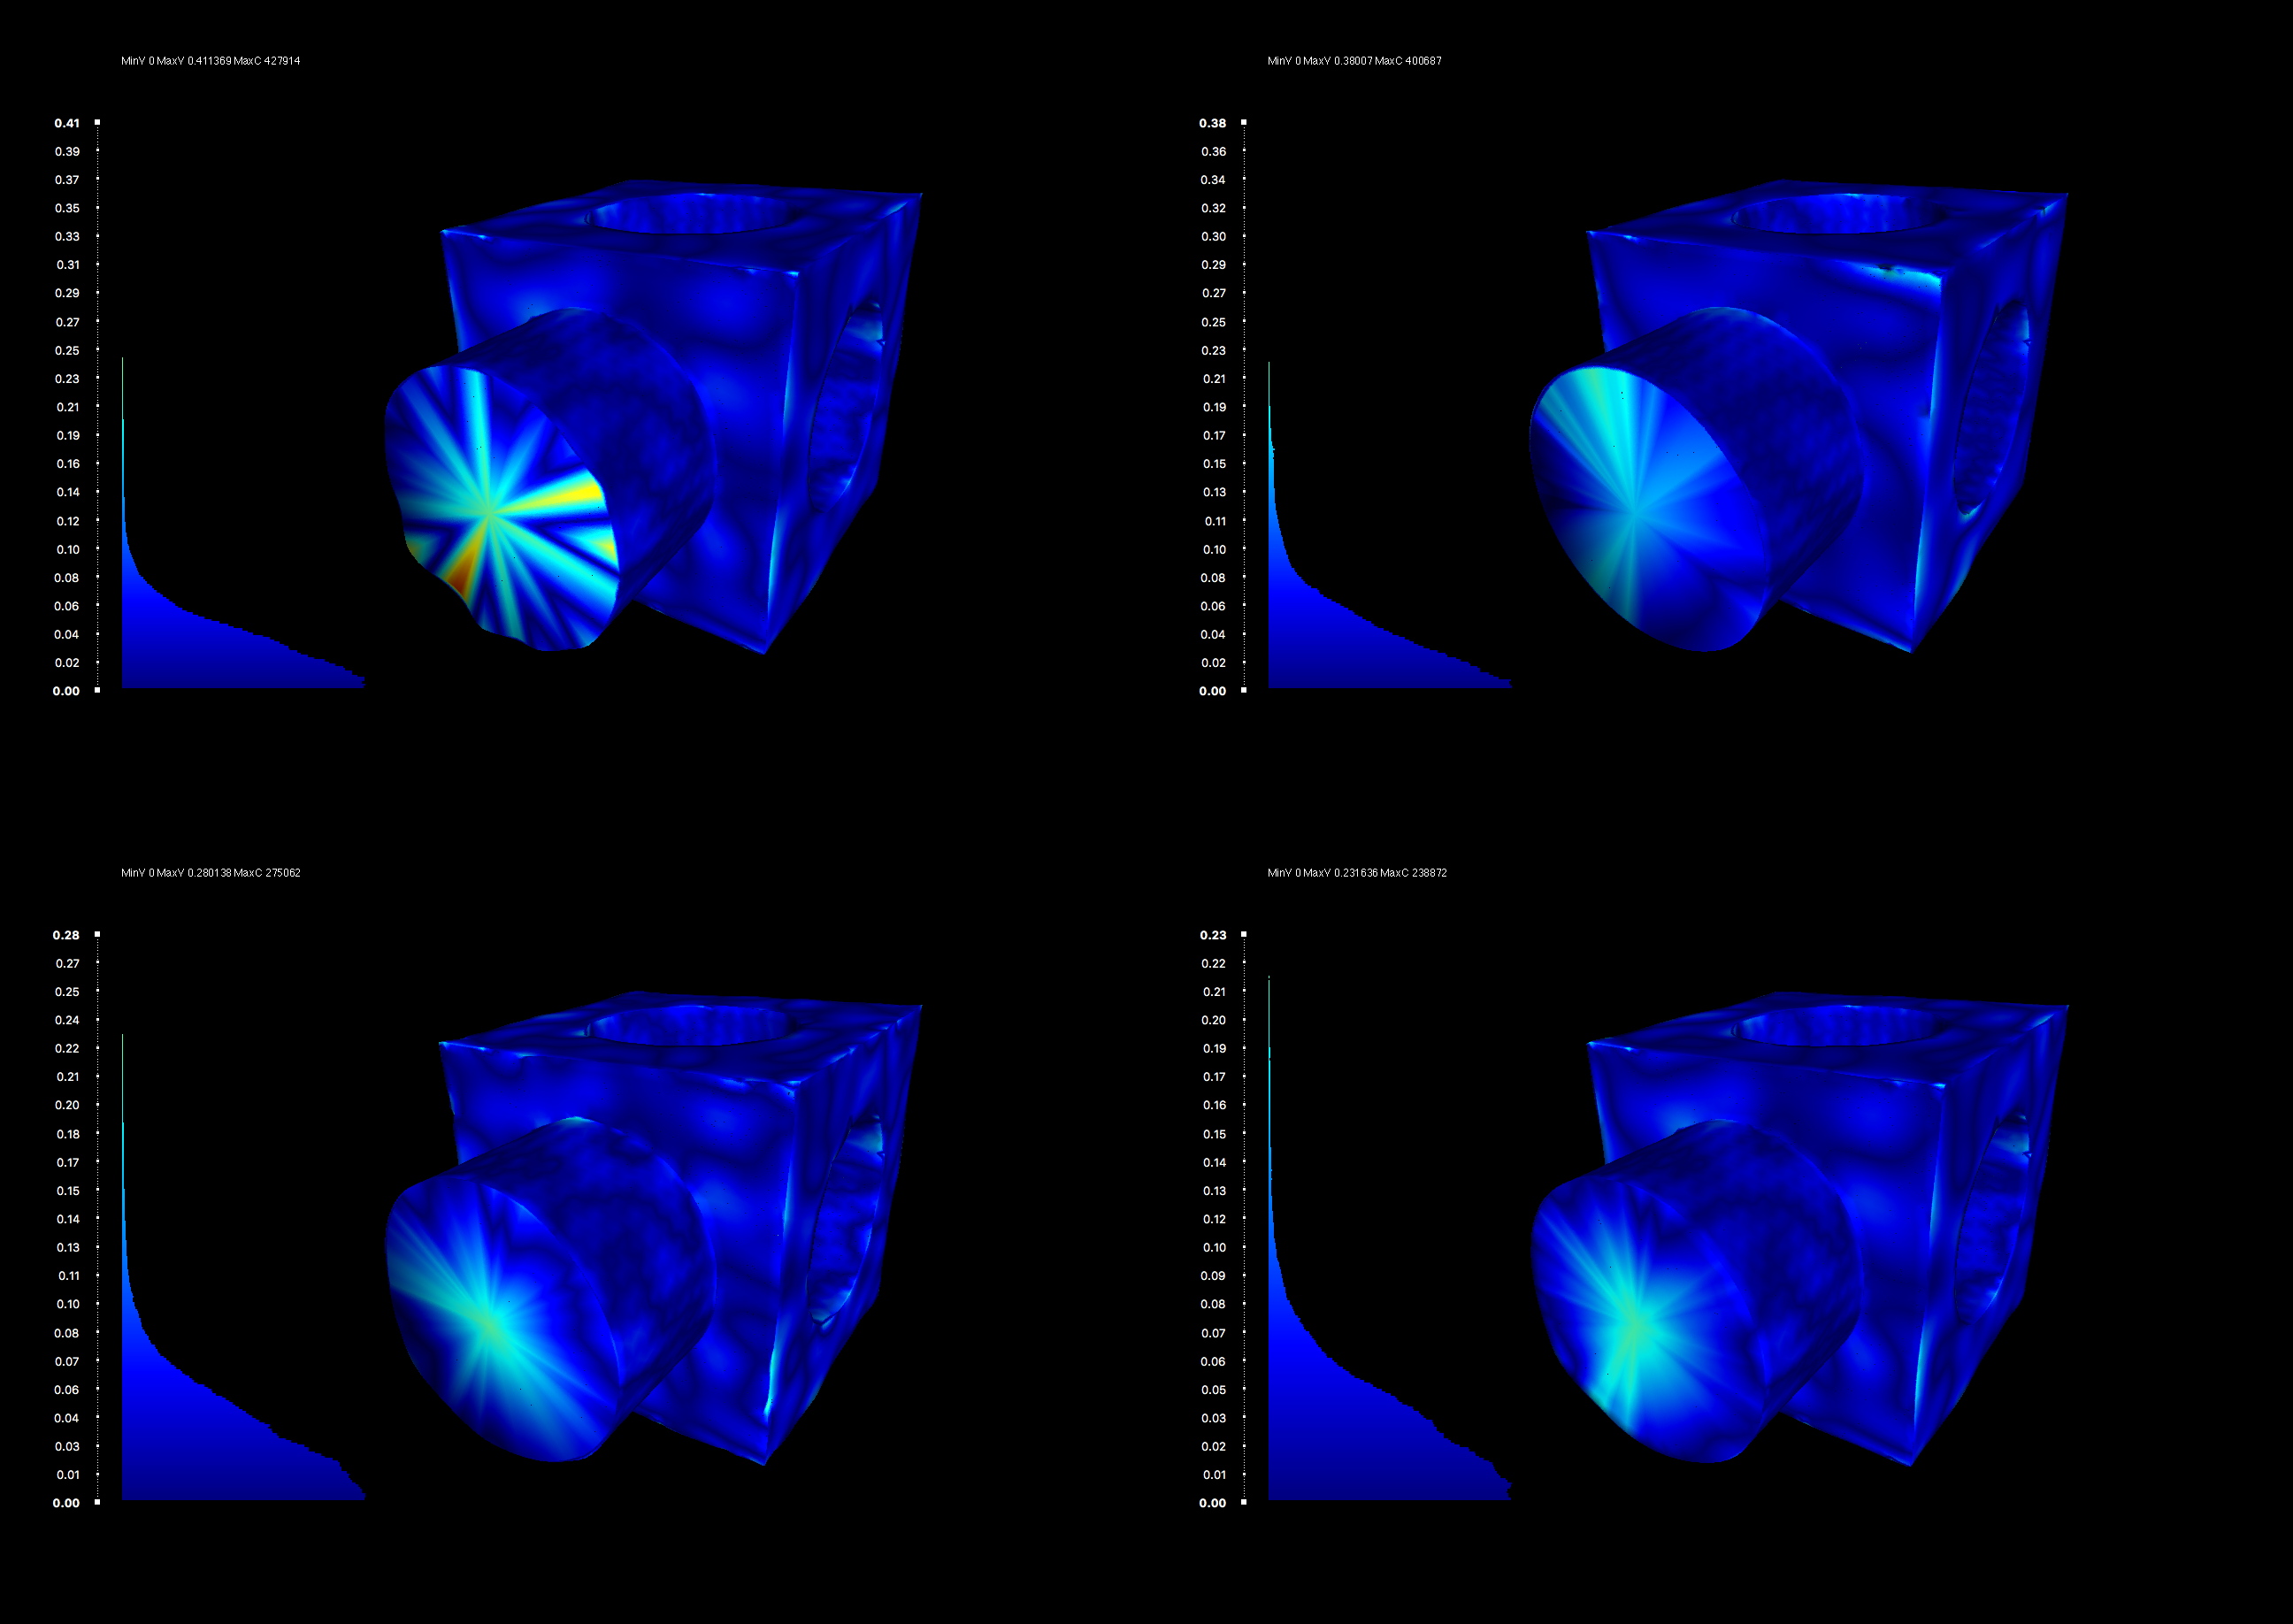
\includegraphics[width=16cm]{figuras/block_hausdorff_final.png}
\caption{Visualização do modelo \textit{block} e um histograma dos 6 milhões de pontos de amostragem e seus respectivos valores de distância de \textit{Hausdorff}. Primeira linha: técnicas de \cite{zhang2015guided} e \cite{sun2007fast}. Segunda linha: técnica \cite{zheng2011bilateral} e a técnica proposta.}
\label{fig:block_hausdorff_final}
\end{figure}

\clearpage


\begin{figure}[p]
\captionsetup{width=\linewidth}
\centering
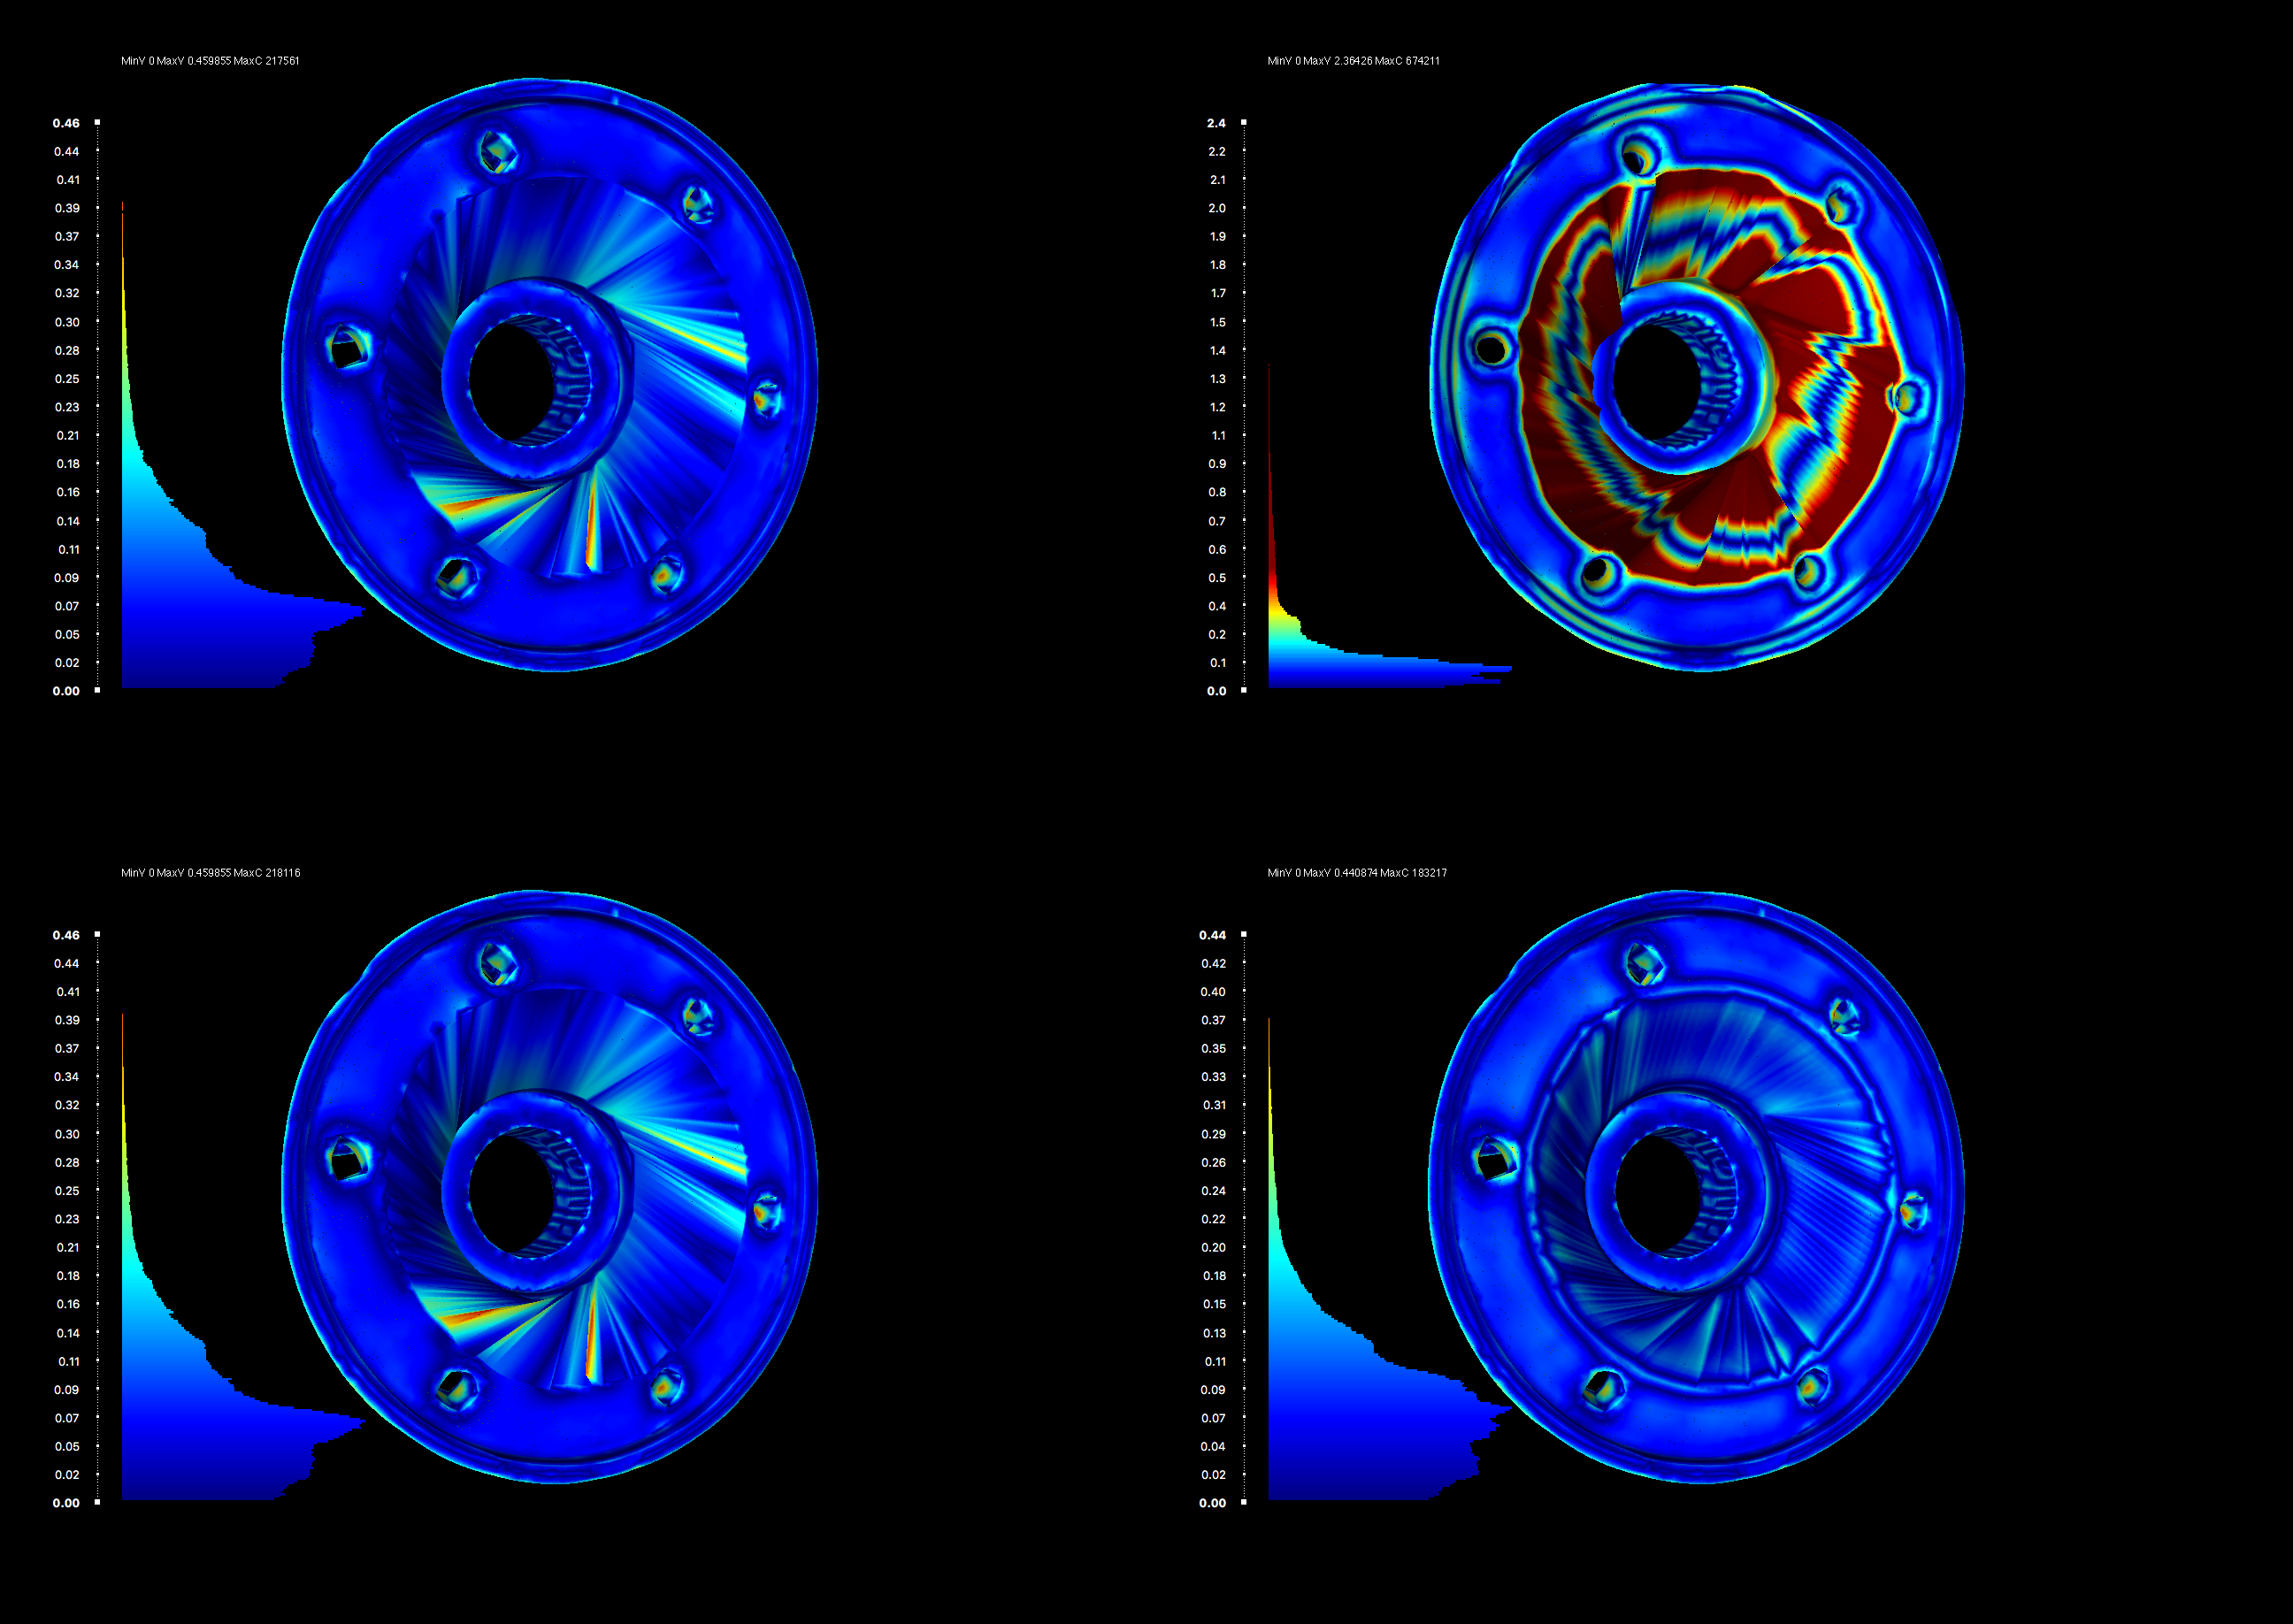
\includegraphics[width=16cm]{figuras/carter_hausdorff_final.png}
\caption{Visualização do modelo \textit{carter} e um histograma dos 6 milhões de pontos de amostragem e seus respectivos valores de distância de \textit{Hausdorff}. Primeira linha: técnicas de \cite{zhang2015guided} e \cite{sun2007fast}. Segunda linha: técnica \cite{zheng2011bilateral} e a técnica proposta.}
\label{fig:carter_hausdorff_final}
\end{figure}

\clearpage


\begin{figure}[p]
\captionsetup{width=\linewidth}
\centering
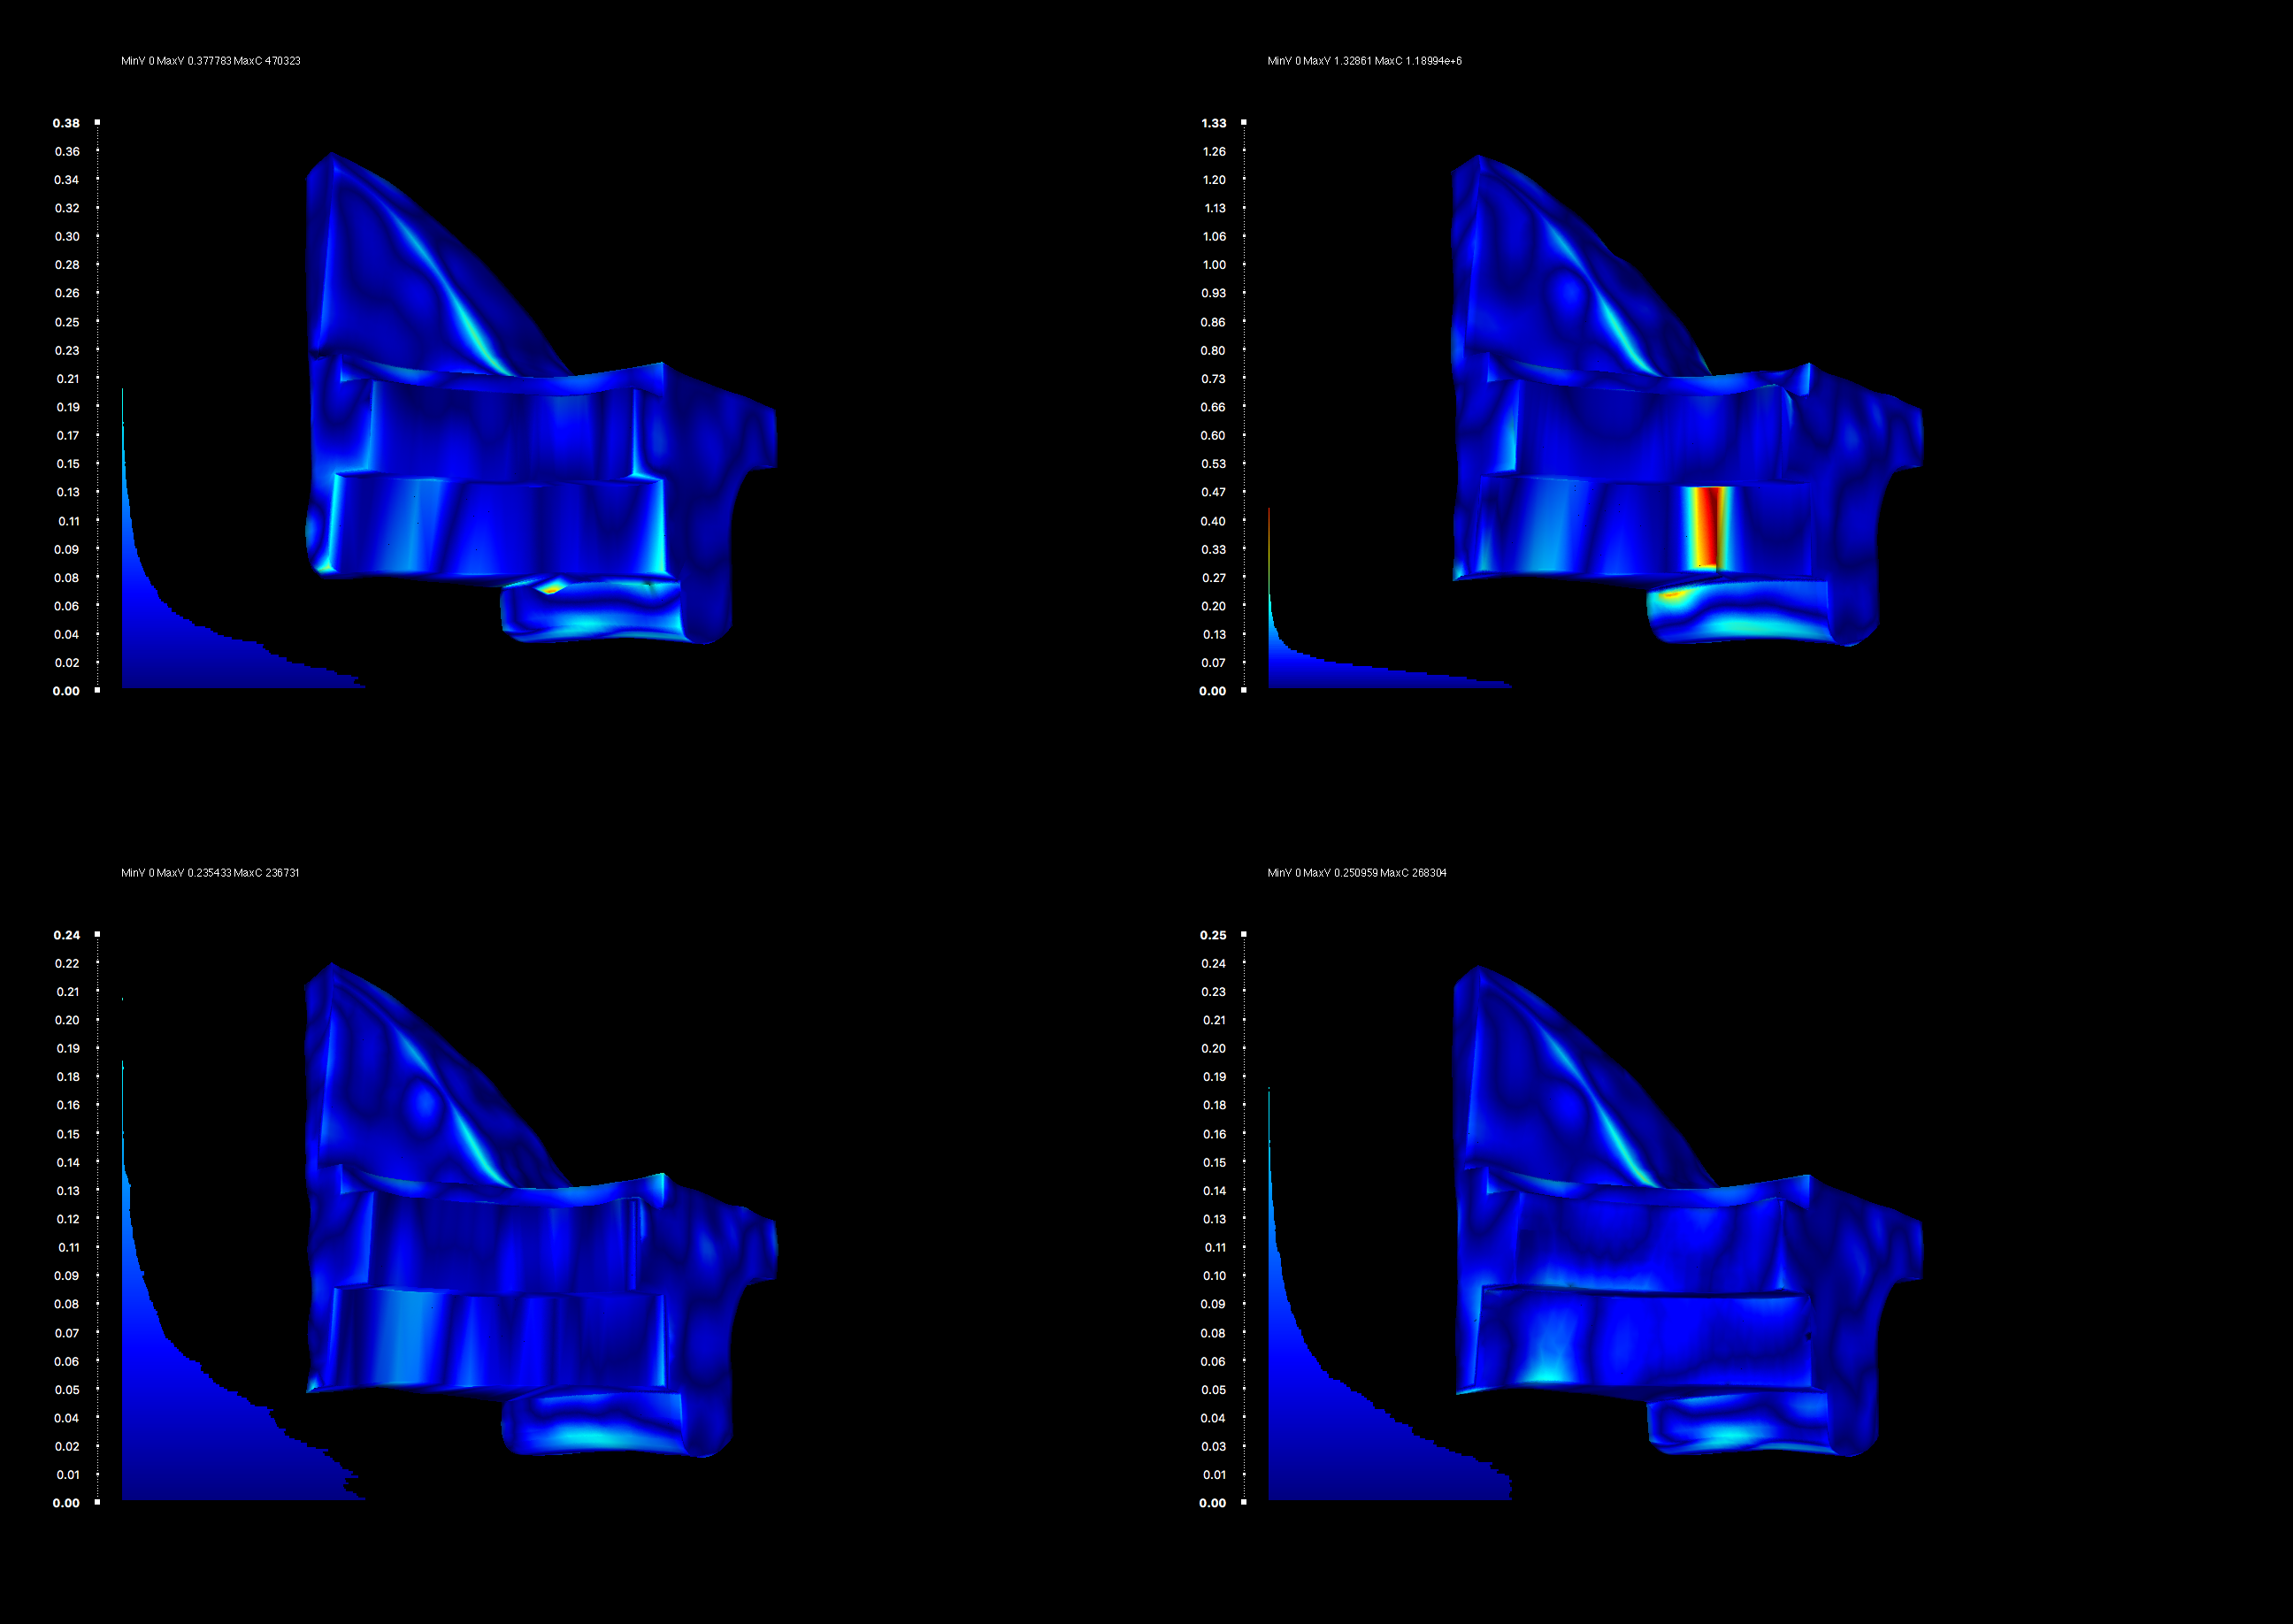
\includegraphics[width=16cm]{figuras/mechanic1_hausdorff_final.png}
\caption{Visualização do modelo \textit{mechanic} e um histograma dos 6 milhões de pontos de amostragem e seus respectivos valores de distância de \textit{Hausdorff}. Primeira linha: técnicas de \cite{zhang2015guided} e \cite{sun2007fast}. Segunda linha: técnica \cite{zheng2011bilateral} e a técnica proposta.}
\label{fig:mechanic1_hausdorff_final}
\end{figure}

\clearpage


\begin{figure}[p]
\captionsetup{width=\linewidth}
\centering
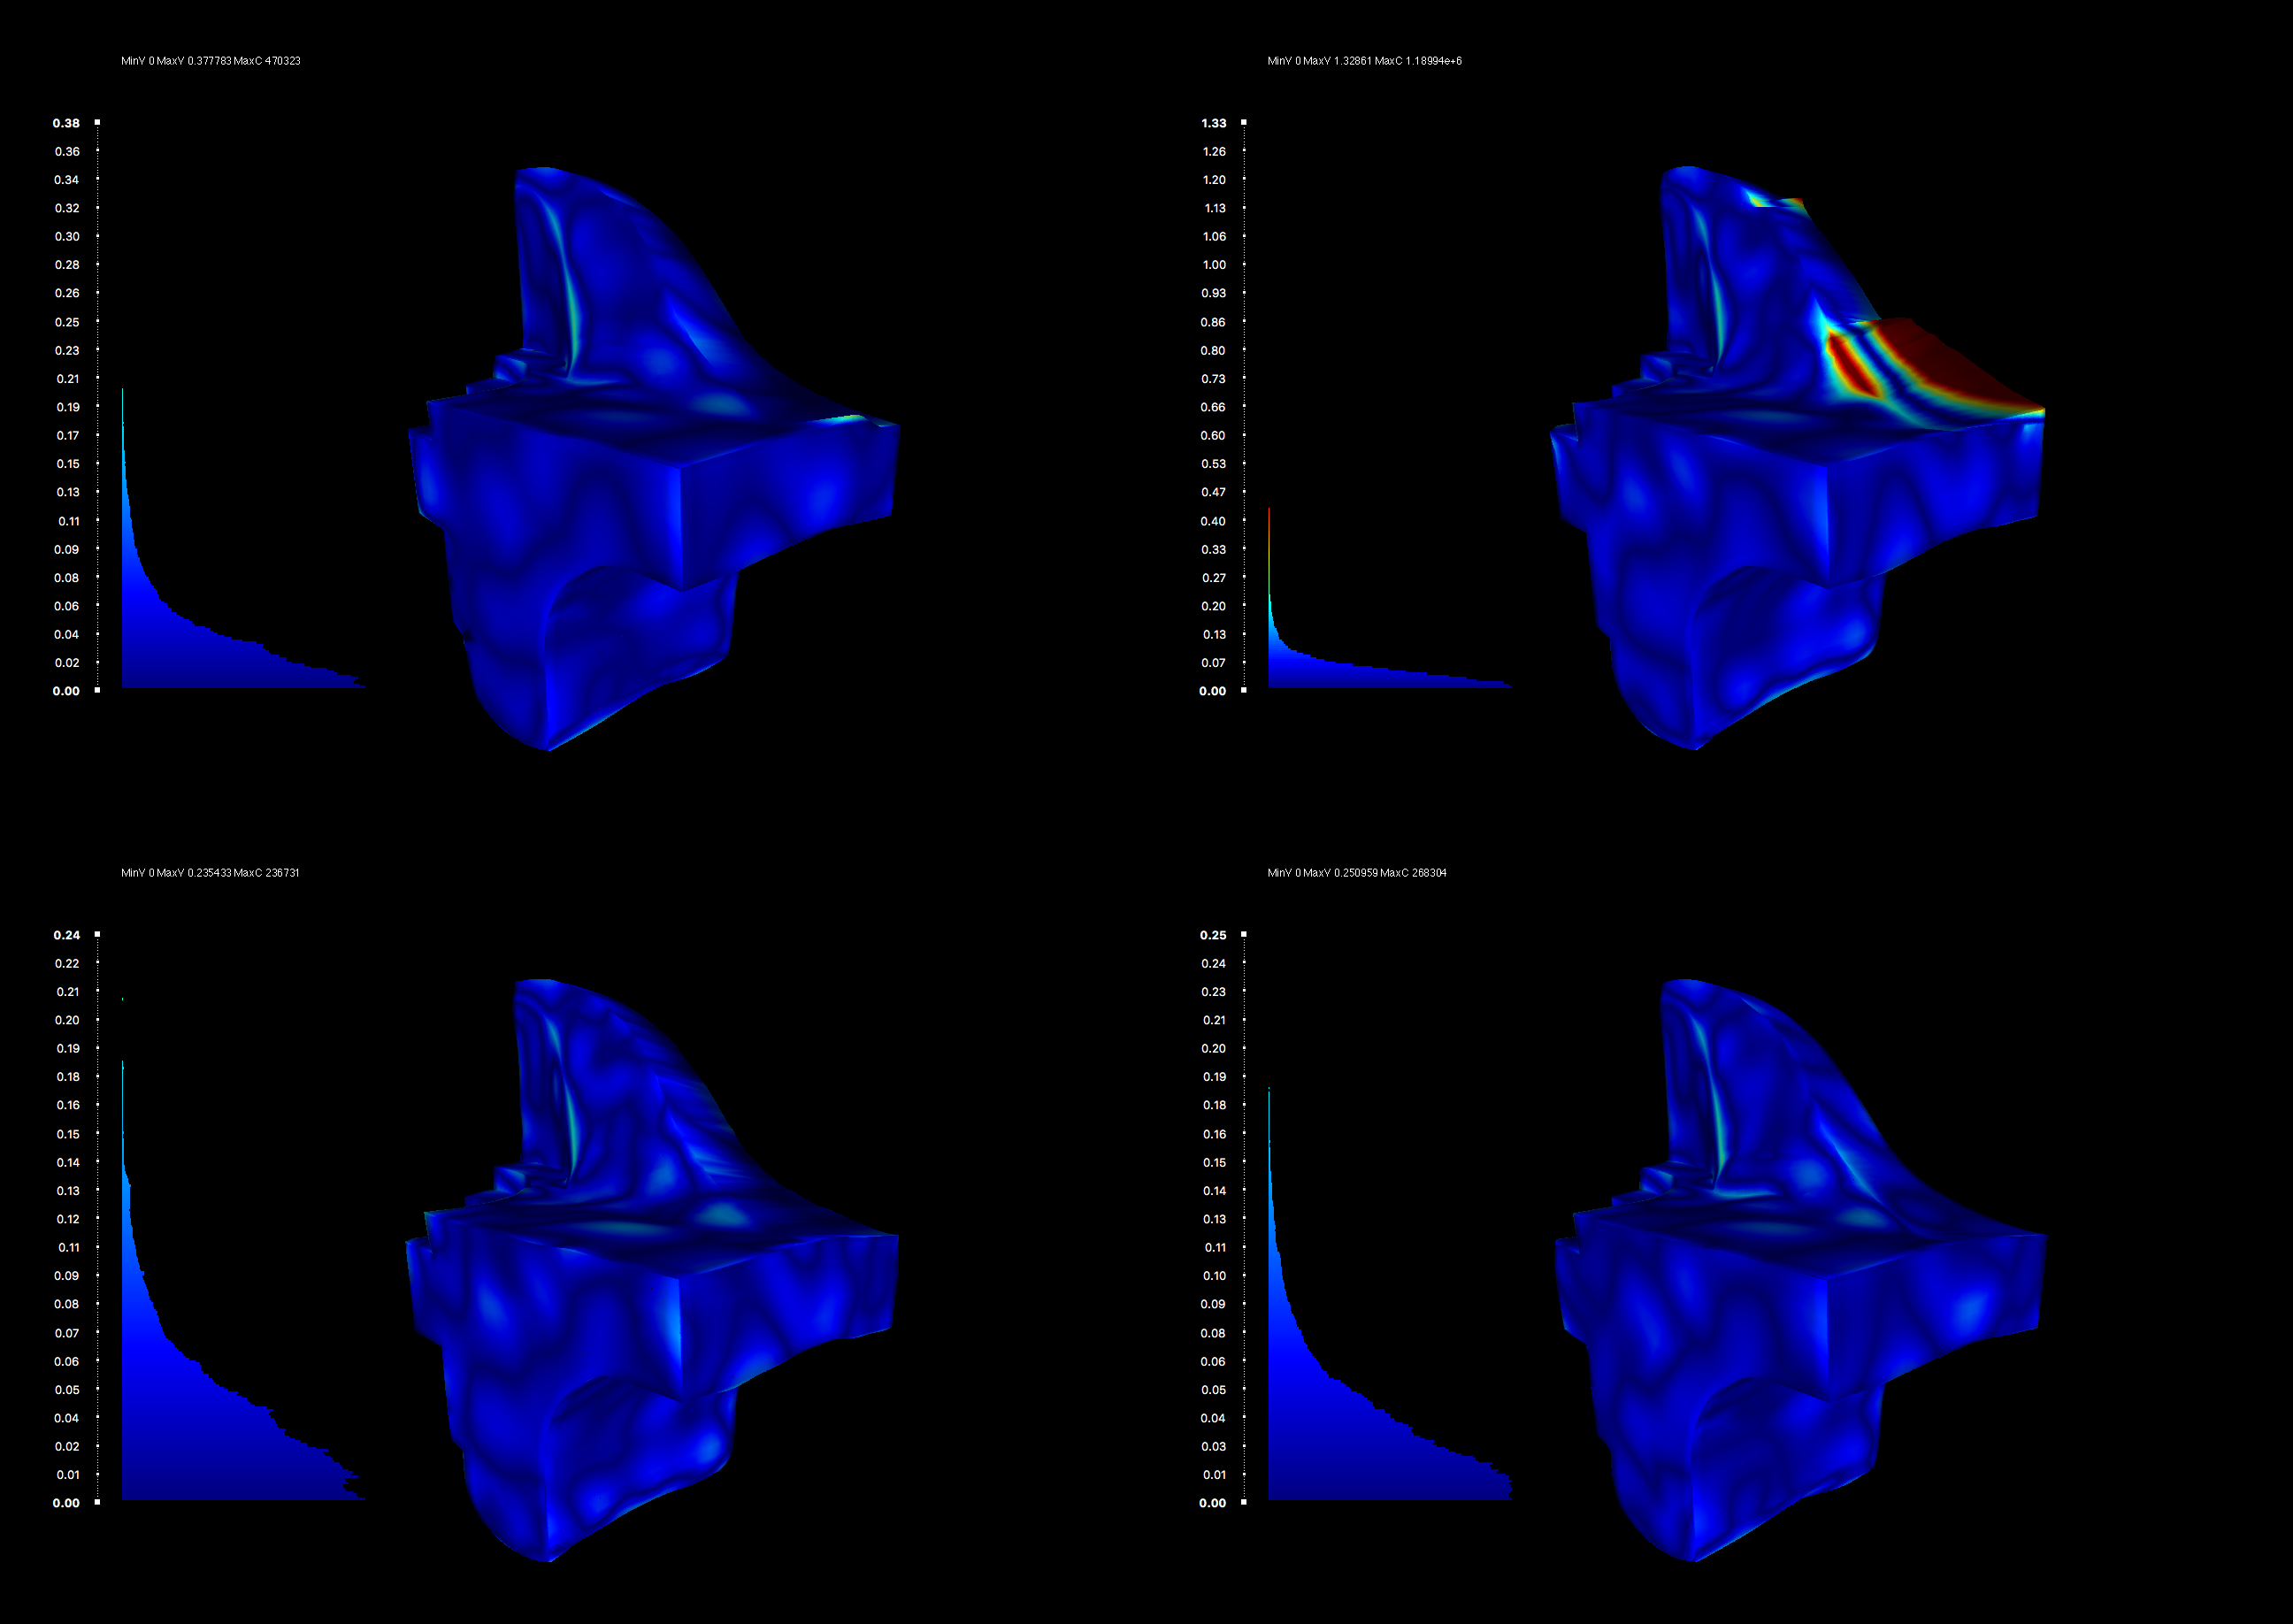
\includegraphics[width=16cm]{figuras/mechanic2_hausdorff_final.png}
\caption{Visualização do modelo \textit{mechanic} e um histograma dos 6 milhões de pontos de amostragem e seus respectivos valores de distância de \textit{Hausdorff}. Primeira linha: técnicas de \cite{zhang2015guided} e \cite{sun2007fast}. Segunda linha: técnica \cite{zheng2011bilateral} e a técnica proposta.}
\label{fig:mechanic2_hausdorff_final}
\end{figure}

\clearpage

\begin{figure}[!h]
\captionsetup{width=\linewidth}
\centering
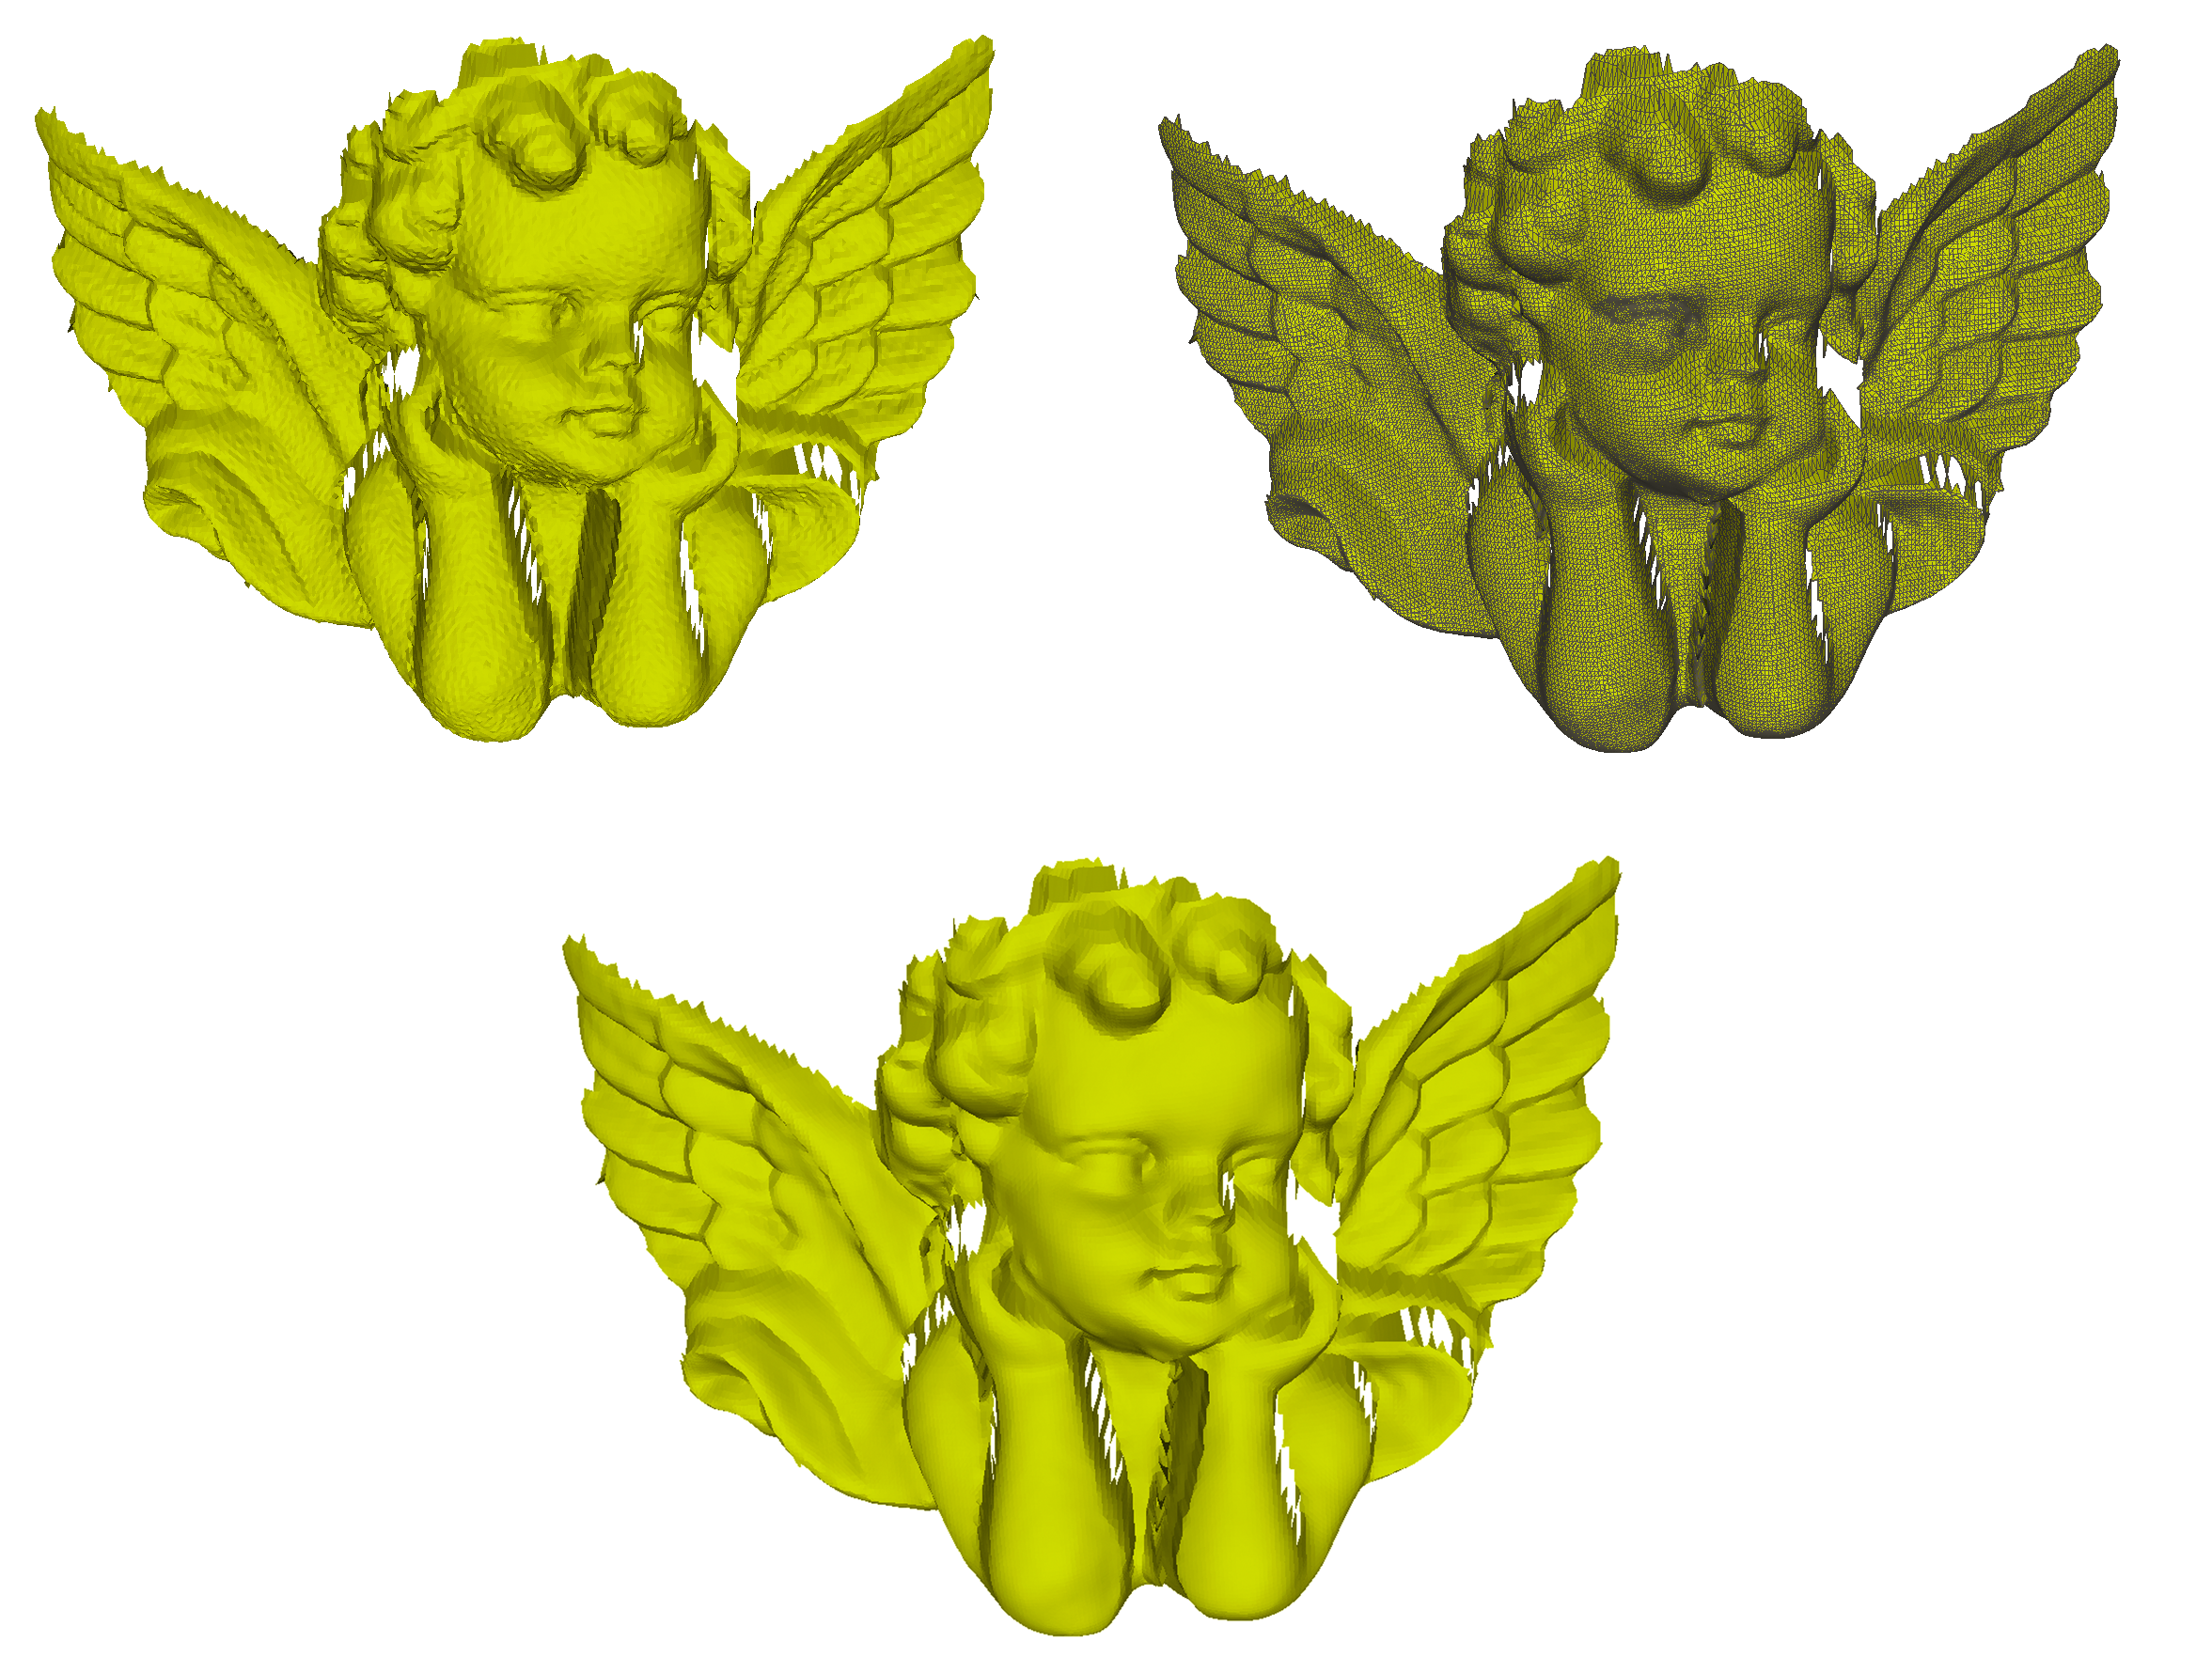
\includegraphics[width=\linewidth]{figuras/angel_final.png}
\caption{Técnica proposta utilizada no modelo \textit{angel}. Acima: modelo \textit{angel} com ruído e ao lado com ruído e malha. Abaixo: o resultado da técnica proposta aplicada ao modelo \textit{angel}.}
\label{fig:angel_final}
\end{figure}

\vspace{10mm}

\begin{figure}[!h]
\captionsetup{width=\linewidth}
\centering
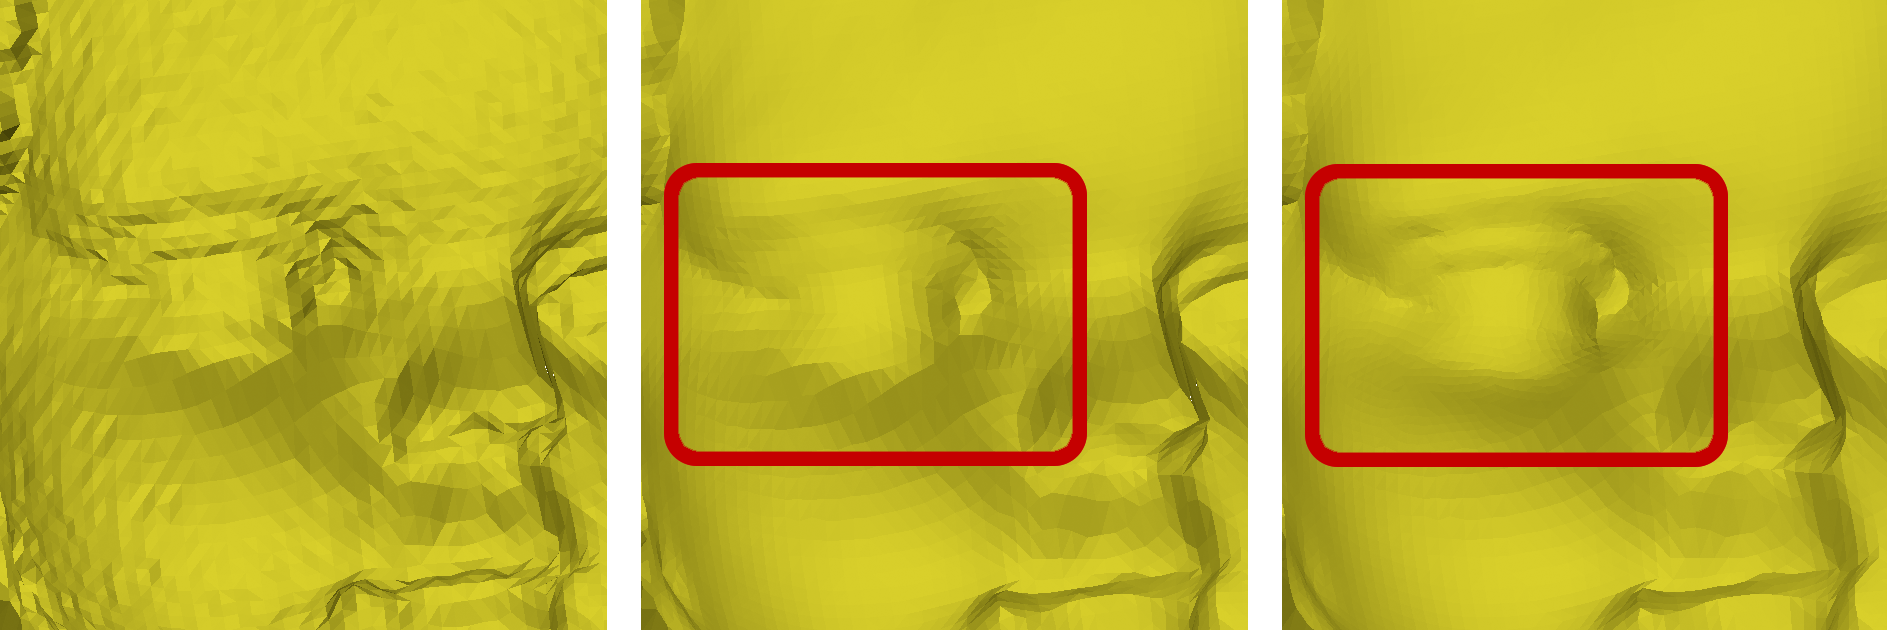
\includegraphics[width=\linewidth]{figuras/angel_detail.png}
\caption{Detalhe da região do olho do modelo \textit{angel}. Da esquerda para a direita: modelo \textit{angel} original com ruído, resultado da técnica proposta sem o passo de pré-processamento, resultado da técnica proposta com passo de pré-processamento.}
\label{fig:angel_detail}
\end{figure}


Pode-se notar, pelas figuras, que a técnica proposta obtém os melhores resultados para todos os modelos. Por fim, uma comparação dos valores das métricas para as quatro técnicas é mostrado na Tabela \ref{table:comparação_métricas}. A técnica proposta obtém melhores resultados para todos os modelos nas métricas mais importantes, obtendo o menor MMHD para todos os modelos apresentados. Em negrito são mostrados os melhores valores encontrados para cada modelo.

\begin{table}[]
\centering
\footnotesize
\renewcommand{\arraystretch}{1.3}
\caption{Comparação da técnica proposta com \cite{zhang2015guided}, \cite{sun2007fast} e \cite{zheng2011bilateral}.}
\setlength\tabcolsep{2pt}
\begin{tabular}{ |c|c|c|c|c|c| } 
\hline
Modelo & Métrica de Erro & \cite{zhang2015guided} & \cite{sun2007fast} & \cite{zheng2011bilateral} & Técnica Proposta \\
\hline
\hline

\multirow{5}{4em}{\centering \textit{Block}} 
& Sample Points & 6000000 & 6000000 & 6000000 & 6000000\\ 
\cline{2-6}
& MHD Mínimo & 0.0 & 0.0 & 0.0 & 0.0\\ 
\cline{2-6}
& MHD Máximo & 0.411390 & 0.380070 & 0.280138 & \textbf{0.231636}\\ 
\cline{2-6}
& \textbf{MMHD} & 0.032300 & 0.35615 & 0.033508 & \textbf{0.031509} \\ 
\cline{2-6}
& Proporção de Volume & 0.997919 & 0.997511 & \textbf{0.998231} & 0.9980328\\ 
\cline{1-6}

\multirow{5}{4em}{\centering \textit{Carter}} 
& Sample Points & 6000000 & 6000000 & 6000000 & 6000000\\ 
\cline{2-6}
& MHD Mínimo & 0.0 & 0.0 & 0.0 & 0.0\\ 
\cline{2-6}
& MHD Máximo & 0.459855 & 2.364260 & 0.459855 & \textbf{0.440874}\\ 
\cline{2-6}
& \textbf{MMHD} & 0.075780 & 0.164315 & 0.075759 & \textbf{0.075653} \\ 
\cline{2-6}
& Proporção de Volume & 1.06965 & \textbf{1.06304} & 1.06965 & 1.06701\\ 
\cline{1-6}

\multirow{5}{4em}{\centering \textit{Mechanic}} 
& Sample Points & 6000000 & 6000000 & 6000000 & 6000000\\ 
\cline{2-6}
& MHD Mínimo & 0.0 & 0.0 & 0.0 & 0.0\\ 
\cline{2-6}
& MHD Máximo & 0.377783 & 1.328610 & \textbf{0.235433} & 0.250672\\ 
\cline{2-6}
& \textbf{MMHD} & 0.032143 & 0.052403 & 0.033874 & \textbf{0.031893} \\ 
\cline{2-6}
& Proporção de Volume & 0.995846 & 1.00102 & \textbf{0.998717} & 0.997236 \\ 
\cline{1-6}

\hline
\end{tabular}
\label{table:comparação_métricas}
\end{table}